\documentclass[../main.tex]{subfiles}
\begin{document}

\headline{Data}
An older version of the \kcite{solc-versions-testset}, commit 923fa5bb5abb2939e54fb5404e9e287b1f0f0cec.
Nine Solidity source files compiled with four solc versions (5, 6, 7, 8) times three optimization
settings (no optimization, runs = 1, runs = 999999).
Necessary changes where made to the source code to ensure compatibility with the different solc
version without altering the function of the contracts.

\headline{Pre-Processing}
The runtime codes where segmented and the first segment skeletonized and then filtered with the following opcode filter. I defined the filter based on my intuition, for wich opcodes are hard to be replaced by others.
\begin{lstlisting}[style=pymd]
(OP.is_log() or OP.is_storage() or OP.is_sys_op() or OP.is_env_info()
  or OP.is_block_info() or OP == opcodes.SHA3 or OP == opcodes.GAS)
\end{lstlisting}
\begin{lstlisting}[style=pysm]
# GASPRICE CALLER SSTORE TIMESTAMP LOG3 ORIGIN INVALID LOG2 ADDRESS BLOCKHASH STATICCALL CALLDATALOAD CALL CALLDATASIZE RETURNDATASIZE EXTCODEHASH GAS LOG0 DIFFICULTY CODESIZE DELEGATECALL CALLVALUE RETURNDATACOPY RETURN NUMBER SELFDESTRUCT CALLCODE REVERT CALLDATACOPY COINBASE EXTCODESIZE CODECOPY CREATE SHA3 LOG4 SLOAD EXTCODECOPY GASLIMIT CREATE2 LOG1 BALANCE
\end{lstlisting}

\headline{Similarity}
Similarity for all code pairs was calculated via Jaccard Index on the bytebags of the filtered codes.

\headline{Clustering}
The clustering \figref{solc_bytebag_cluster} was done in Gephi (0.9.2) with the settings \figref{solc_bytebag_cluster_settings}.
Nodes with the same color have the same source code.
The graph is fully connected and the edge weights are determined by the similarity scores of the pairs.

\begin{figure*}[ht!]
  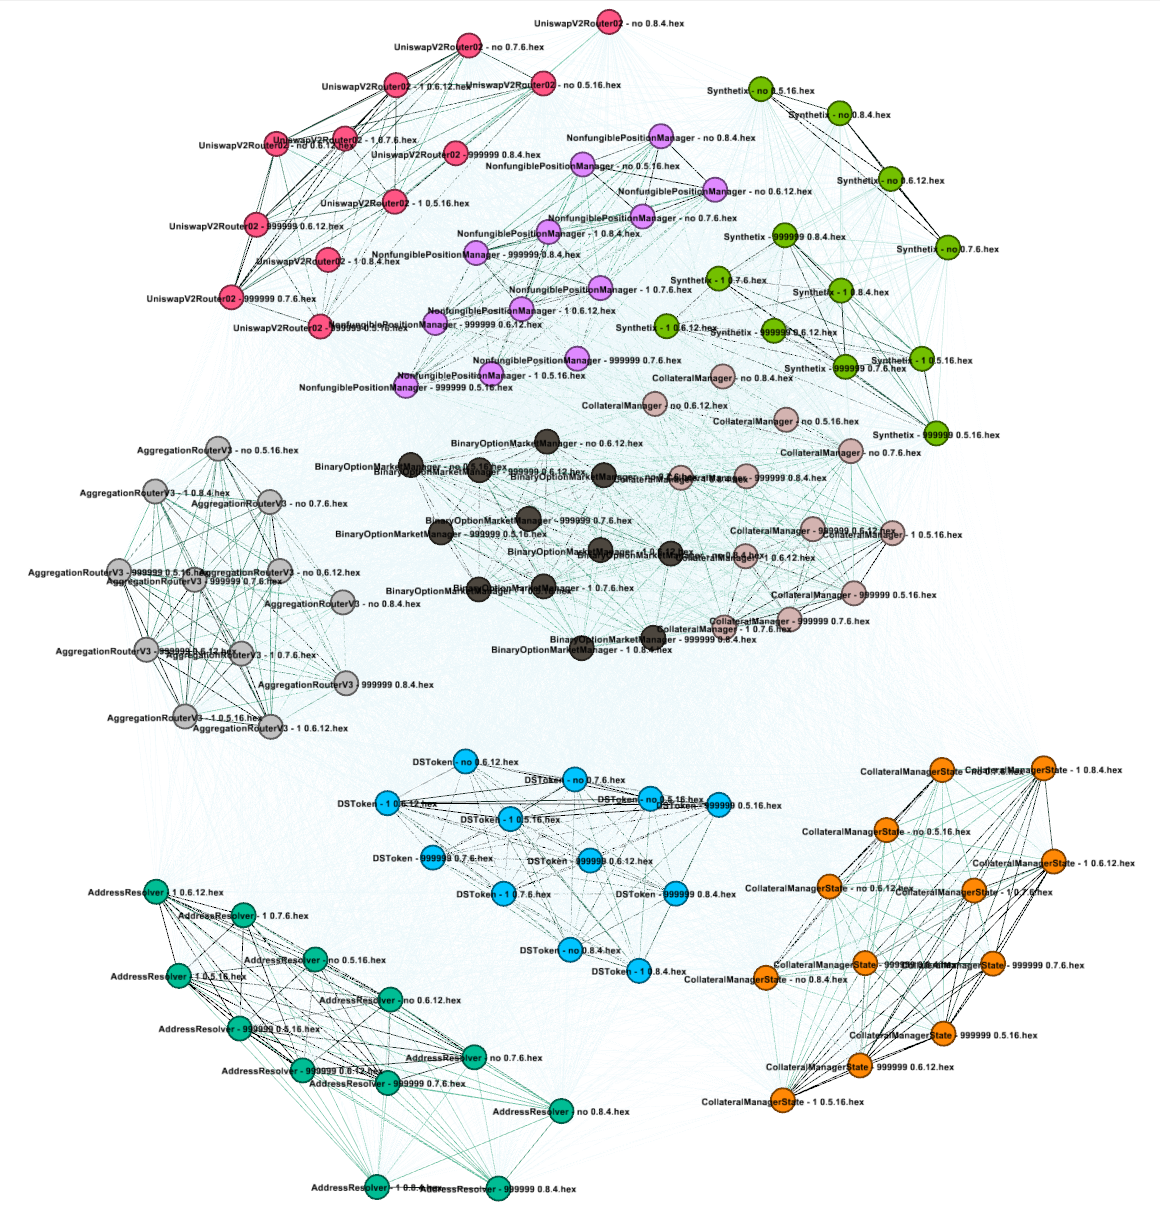
\includegraphics[width=\linewidth]{../../bsc-notes/clustering/clustering_result_many_solc_versions_byteBag_significant_only_2021-06-06_163755.png}
  \caption{solc versions bytebag}
  \label{fig:solc_bytebag_cluster}
\end{figure*}

\begin{figure*}[ht!]
  \centering
  \includegraphics[width=10cm]{../../bsc-notes/clustering/clustering_settings_many_solc_versions_byteBag_significant_only_2021-06-06_163526.png}
  \caption{Gephi settings}
  \label{fig:solc_bytebag_cluster_settings}
\end{figure*}

\headline{Observation}
The clustering algo formed cohesive clusters, mostly due to the fact that the dataset is small and the contracts differ significantly in size alone.
Nonetheless, noticeable is that the Synthetix codes without optimization from all 4 solc versions form a cluster separate from the other Synthetix codes. The no optimization variants in the CollateralManagerState cluster also group tightly \figref{CollateralManagerState}.

\begin{figure*}[ht!]
  \centering
  \includegraphics[width=14cm]{../../bsc-notes/clustering/clustering_result_CollateralManagerState_many_solc_versions_byteBag_significant_only _2021-06-06_163626.png}
  \caption{CollateralManagerState}
  \label{fig:CollateralManagerState}
\end{figure*}

\headline{Analysis}
When comparing the frequency of the opcodes in \code{Synthetix - no 0.8.4.hex} and\\
\code{Synthetix - 999999 0.8.4.hex} these 7 op-codes show the highest change \tblref{opt_diff}.

\begin{table}[ht!]
  \centering
  \csvreader[
    tabular=rrlrrr,
    table head= dec & hex & op-code & no 0.8.4 & 999999 0.8.4 & diff\\\hline,
    head to column names]{csv/opt_diff.csv}{}{%
      \csvcoli & \texttt{\csvcolii} & \csvcoliii & \csvcoliv & \csvcolv & \csvcolvi}
  \caption{optimization differences}
  \label{tbl:opt_diff}
\end{table}

\code{54 0x36 CALLDATASIZE} is the most consistent across solc versions and optimization settings.

\code{59 0x3B EXTCODESIZE} is also very consistent.

\code{90 0x5A GAS} has a high absolute difference between the Synthetix contracts but it has higher differences across contracts.

\headline{Interpretation}
Many of the opcodes, I thought significant show hight changes in frequency when optimization is applied, especially the \code{RETURN} opcode should not be included in the filter, since optimization drastically reduces its prevalence from 45 to 1.
Manually analysis optimization options change the codes more than solc version changes.

\end{document}
